\documentclass[handout]{beamer}
\usetheme{Copenhagen}
\usecolortheme{crane}
\usepackage[utf8]{inputenc}
\usefonttheme{structuresmallcapsserif}
\usepackage{lmodern, kotex, babel, graphicx, cancel}
\usepackage[showdow]{datetime2}

\newcommand*{\datefmt}[3]{%
  \number#3~\pgfcalendarmonthname{#2} \number#1%
}

\title{Workbook Examples \\ Chapter $3$ \\ Math $1100$}
\author{Don D. Kim}
%\institute{\Large{\textsc{University of Missouri}}}
\date{\datefmt{\year}{\month}{\day}}

\titlegraphic{\vfill \centering 
\includegraphics[scale=1.0]{Mizzou.png}\vfill}

\begin {document}

\begin{frame}
	\titlepage
\end{frame}

\begin{frame}
	\frametitle{Outline}
	\tableofcontents
\end{frame}

\section{$\S 3.2$: Quadratic Equations, Functions, Zeros, \& Models}

\begin{frame}
	\frametitle{Example}
	\begin{enumerate}
		\item[]<1-> Solve \[ 2x^{2}-x=3. \]
		\item[]<2->\textsc{Solution:}
		\item[]<3-> \[ \Rightarrow 2x^{2}-x-3=0 \]
		\item[]<4->\[ \Rightarrow (2x-3)(x+1)=0 \]
		\item[]<5->\[ \Rightarrow 2x-3=0, x+1=0 \]
		\item[]<6->\[ \Rightarrow x=\frac{3}{2}, x=-1\]
	\end{enumerate}
\end{frame}

\begin{frame}
	\frametitle{Example}
	\begin{enumerate}
		\item[]<1-> Solve \[ 2x^{2}-10=0. \]
		\item[]<2->\textsc{Solution:}
		\item[]<3->\[ \Rightarrow 2x^{2}=10\]
		\item[]<4->\[\Rightarrow x^{2}=5\]
		\item[]<5->\[ \Rightarrow x=\pm \sqrt{5} \]
	\end{enumerate}
\end{frame}

\begin{frame}
	\frametitle{Example}
	\begin{enumerate}
		\item[]<1->Solve \[ 4x^{2}=12. \]
		\item[]<2->\textsc{Solution:}
		\item[]<3-> \[ \Rightarrow x^{2}=\frac{12}{4}=3 \]
		\item[]<4->\[ \Rightarrow x=\pm \sqrt{3}. \]
	\end{enumerate}
\end{frame}

\begin{frame}
	\frametitle{Example}
	\begin{enumerate}
		\item[]<1->Find the zeros of
		\item[]<2-> \[ f(x)=x^{2}-6x-10 \]
		\item[]<3-> by completing the square.
		\item[]<4-> \textsc{Solution:}
		\item[]<5-> Set $f(x)=0$, finding
		\item[]<6-> \[ x^{2}-6x-10=0 \]
		\item[]<7-> \[ \Rightarrow x^{2}-6x=10 \]
		\item[]<8->\[ \Rightarrow x^{2}-6x+9=10+9=19 \]
	\end{enumerate}
\end{frame}

\begin{frame}
	\frametitle{Example (cont.)}
	\begin{enumerate}
		\item[]<1->\[ \Rightarrow (x-3)^{2}=19 \]
		\item[]<2->\[ \Rightarrow x-3=\pm \sqrt{19} \]
		\item[]<3->\[ \Rightarrow x=3 \pm \sqrt{19} \]
	\end{enumerate}
\end{frame}

\begin{frame}
	\frametitle{Example}
	\begin{enumerate}
		\item[]<1-> Find the zeros of
		\item[]<2->\[ f(x)=x^{2}-3x-3 \]
		\item[]<3->by completing the square.
		\item[]<4->\textsc{Solution:}
		\item[]<5-> \[ \Rightarrow x^{2}-3x-3=0 \]
		\item[]<6-> \[ \Rightarrow x^{2}-3x=3 \]
		\item[]<7-> \[ \Rightarrow x^{2}-3x+\left( -\frac{3}{2}\right)^{2}=3+\frac{9}{4}=\frac{21}{4} \]
	\end{enumerate}
\end{frame}

\begin{frame}
	\frametitle{Example (cont.)}
	\begin{enumerate}
		\item[]<1-> \[ \Rightarrow \left( x-\frac{3}{2} \right)^{2}=\frac{21}{4} \]
		\item[]<2-> \[ \Rightarrow x-\frac{3}{2}=\pm \sqrt{\frac{21}{4}} \]
		\item[]<3->\[ \Rightarrow x=\frac{3}{2} \pm \frac{\sqrt{21}}{2} \]
	\end{enumerate}
\end{frame}

\begin{frame}
	\frametitle{Example}
	\begin{enumerate}
		\item[]<1->Find the zeros of
		\item[]<2-> \[ 2x^{2}-3x-1=0 \]
		\item[]<3->by completing the square.
		\item[]<4->\textsc{Solution:}
		\item[]<5->\[ \Rightarrow 2\left( x^{2}-\frac{3}{2}x\right)=1\]
		\item[]<6->\[ \Rightarrow 2\left( x^{2}-\frac{3}{2}x+\frac{9}{16}\right)=1+\frac{18}{16} \]
		\item[]<7-> \[ \Rightarrow 2\left( x-\frac{3}{4} \right)^{2}=\frac{17}{8} \]
	\end{enumerate}
\end{frame}

\begin{frame}
	\frametitle{Example (cont.)}
	\begin{enumerate}
		\item[]<1-> \[ \Rightarrow \left( x-\frac{3}{4} \right)^{2}=\frac{17}{16} \]
		\item[]<2-> \[ \Rightarrow x-\frac{3}{4}=\pm \sqrt{\frac{17}{16}}\]
		\item[]<3-> \[ \Rightarrow x=\frac{3 \pm \sqrt{17}}{4}  \]
	\end{enumerate}
\end{frame}

\begin{frame}
	\frametitle{Example}
	\begin{enumerate}
		\item[]<1-> Solve \[ 3x^{2}+2x=7. \]
		\item[]<2-> \textsc{Solution:}
		\item[]<3-> \[ \Rightarrow 3x^{2}+2x-7=0 \]
		\item[]<4-> \[ \Rightarrow a=3, b=2, c=-7 \]
		\item[]<5-> \[ \Rightarrow x=\frac{-2 \pm \sqrt{2^{2}-4(3)(-7)}}{2(3)}\]
		\item[]<6-> \[ \Rightarrow x=\frac{-1 \pm \sqrt{22}}{3}\]
	\end{enumerate}
\end{frame}

\begin{frame}
	\frametitle{Example}
	\begin{enumerate}
		\item[]<1-> Solve \[ 2x^{2}-3x-2=0. \]
		\item[]<2-> \textsc{Solution:}
		\item[]<3-> \[ \Rightarrow a=2, b=-3, c=-2 \]
		\item[]<4-> \[ \Rightarrow  x=\frac{-(-3)\pm \sqrt{(-3)^{2}-4(2)(-2)}}{2(2)}\]
		\item[]<5-> \[ \Rightarrow x=\frac{3 \pm 5}{4}\]
		\item[]<6-> \[ \Rightarrow x=-\frac{1}{2}, 2\]
	\end{enumerate}
\end{frame}

\begin{frame}
	\frametitle{Example}
	\begin{enumerate}
		\item[]<1->Solve \[ 3x^{2}+8x+3=0. \]
		\item[]<2->\textsc{Solutoin:}
		\item[]<3->\[ \Rightarrow x=\frac{-8 \pm \sqrt{64-4(3)(3)}}{2(3)} \]
		\item[]<4-> \[ \Rightarrow x=\frac{-8 \pm 2\sqrt{7}}{6} \]
		\item[]<5-> \[ \Rightarrow x=\frac{-4 \pm \sqrt{7}}{3} \]
	\end{enumerate}
\end{frame}

\begin{frame}
	\frametitle{Example}
	\begin{enumerate}
		\item[]<1-> Solve \[ x^{2}+1=x. \]
		\item[]<2->\textsc{Solution:}
		\item[]<3-> \[ \Rightarrow x^{2}-x+1=0 \]
		\item[]<4-> \[ \Rightarrow x=\frac{1\pm \sqrt{1-4(1)(1)}}{2}\]
		\item[]<5-> \[ \Rightarrow x=\frac{1 \pm \sqrt{3} i}{2}\]
	\end{enumerate}
\end{frame}

\begin{frame}
	\frametitle{Example}
	\begin{enumerate}
		\item[]<1->Solve \[ x^{4}-5x^{2}+4=0. \]
		\item[]<2->\textsc{Solution:} Let $u=x^{2}$.
		\item[]<3-> \[ \Rightarrow u^{2}-5u+4=0 \]
		\item[]<4->\[ \Rightarrow (u-4)(u-1)=0\]
		\item[]<5->\[ \Rightarrow u=4, u=1 \]
		\item[]<6-> \[ \Rightarrow x^{2}=4, x^{2}=1 \]
		\item[]<7-> \[ \Rightarrow x=\pm 1, \pm 2 \]
	\end{enumerate}
\end{frame}

\begin{frame}
	\frametitle{Example}
	\begin{enumerate}
		\item[]<1-> Solve \[ x^{4}-3x^{2}+2=0. \]
		\item[]<2-> \textsc{Solution:} Let $u=x^{2}$.
		\item[]<3-> \[ \Rightarrow u^{2}-3u+2=0 \]
		\item[]<4-> \[ \Rightarrow (u-2)(u-1)=0 \]
		\item[]<5-> \[ \Rightarrow u=2, u=1 \]
		\item[]<6-> \[ \Rightarrow x^{2}=2, x^{2}=1 \]
		\item[]<7-> \[ \Rightarrow x=\pm \sqrt{2}, \pm 1 \]
	\end{enumerate}
\end{frame}

\begin{frame}
	\frametitle{Example}
	\begin{enumerate}
		\item[]<1-> Solve \[ 4t^{3}-27t=-12t^{2}. \]
		\item[]<2-> \textsc{Solution:}
		\item[]<3-> \[ \Rightarrow 4t^{3}+12t^{2}-27t=0 \]
		\item[]<4-> \[ \Rightarrow t(4t^{2}+12t-27)=0 \]
		\item[]<5-> \[ \Rightarrow t(2t-3)(2t+9)=0 \]
		\item[]<6-> \[ \Rightarrow t=0, 2t-3=0, 2t+9=0 \]
		\item[]<7-> \[ \Rightarrow t=0, \frac{3}{2}, -\frac{9}{2} \]
	\end{enumerate}
\end{frame}

\begin{frame}
	\frametitle{Example}
	\begin{enumerate}
		\item[]<1-> Solve \[ 18x^{3}+15x^{2}+12x+10=0. \]
		\item[]<2-> \textsc{Solution:}
		\item[]<3-> \[ \Rightarrow 3x^{2}(6x+5)+2(6x+5)=0 \]
		\item[]<4-> \[ \Rightarrow (6x+5)(3x^{2}+2)=0 \]
		\item[]<5-> \[ \Rightarrow x=-\frac{5}{6}, \pm \sqrt{\frac{2}{3}} i \]
	\end{enumerate}
\end{frame}

\begin{frame}
	\frametitle{Example}
	\begin{enumerate}
		\item[]<1->Solve \[ 9x^{3}+x^{2}-9x-1=0. \]
		\item[]<2-> \textsc{Solution:}
		\item[]<3-> \[ \Rightarrow x^{2}(9x+1)-(9x+1)=0\]
		\item[]<4-> \[ \Rightarrow (9x+1)(x^{2}-1)=0 \]
		\item[]<5-> \[ \Rightarrow x=-\frac{1}{9}, \pm 1 \]
	\end{enumerate}
\end{frame}

\section{$\S3.3$ Analyzing Graphs of Quadratic Functions}

\begin{frame}
	\frametitle{Example}
	\begin{enumerate}
		\item[]<1-> Given the graph below, a graph of the quadratic function $f(x)=a(x-h)^{2}+k$, find the vertex, the axis of symmetry, and the minimum or maximum value of the function.
		\item[]<2->
			\begin{center}
				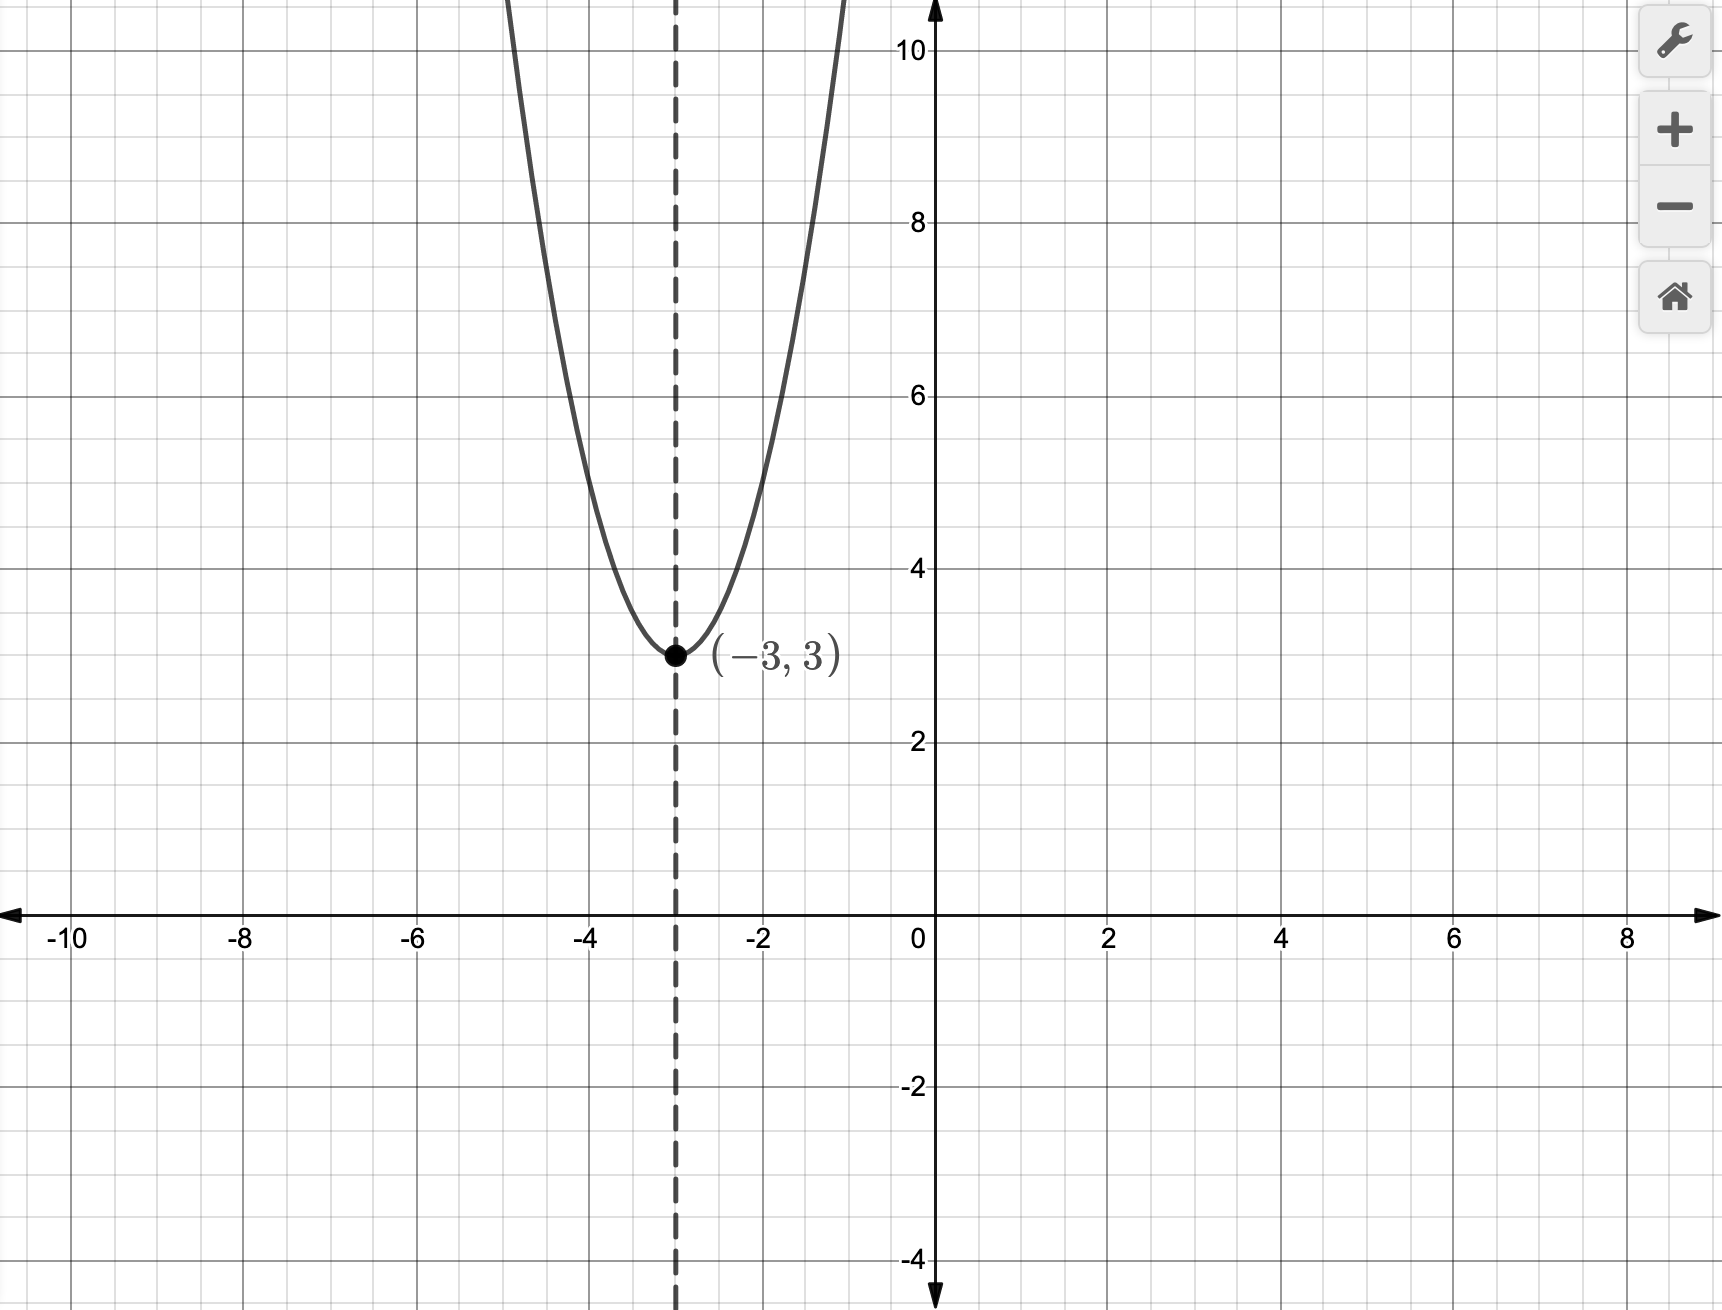
\includegraphics[scale=0.2]{3_3_1.png}
			\end{center}
	\end{enumerate}
\end{frame}

\begin{frame}
	\frametitle{Example (cont.)}
	\begin{enumerate}
		\item[]<1-> \textsc{Solution:}
		\item[]<2-> The vertex is $V=(-3,3)$.
		\item[]<3-> The axis of symmetry is $x=-3$.
		\item[]<4-> The function has a minimum of $y=3$.
	\end{enumerate}
\end{frame}

\begin{frame}
	\frametitle{Example}
	\begin{enumerate}
		\item[]<1-> Find the vertex, the axis of symmetry, and the maximum or minimum value of
		\item[]<2->\[ f(x)=x^{2}+10x+28. \]
		\item[]<3-> \textsc{Solution:}
		\item[]<4-> The vertex is $V=\left( -\frac{10}{2(1)}, f \left( -\frac{10}{2(1)} \right)\right)=( -5,3 )$.
		\item[]<5-> The axis of symmetry is $x=-5$.
		\item[]<6-> The function has a minimum of $y=-5$.
	\end{enumerate}
\end{frame}

\begin{frame}
	\frametitle{Example (cont.)}
	\begin{enumerate}
		\item[]<1-> The graph of the function is
		\item[]<2->\begin{center}
				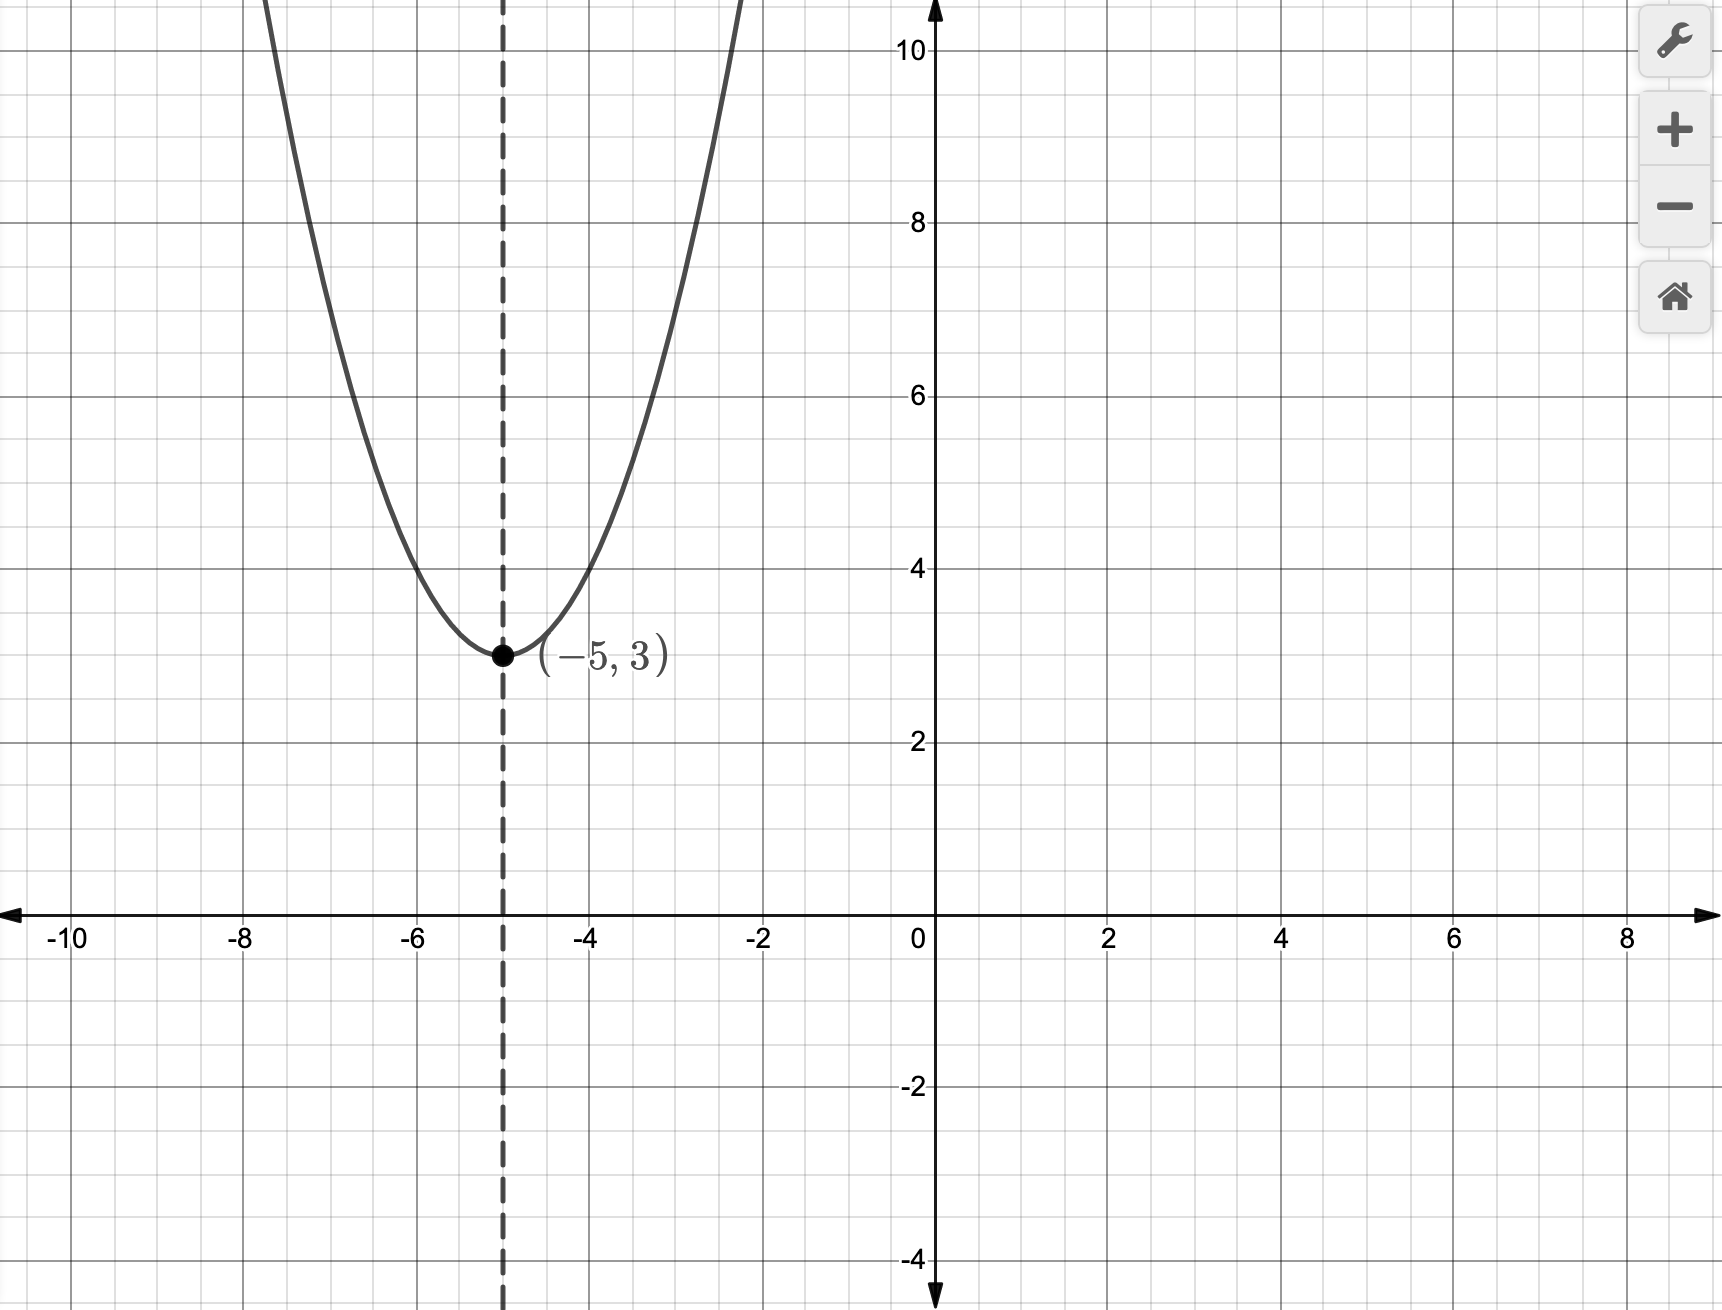
\includegraphics[scale=0.25]{3_3_2.png}
			\end{center}
	\end{enumerate}
\end{frame}

\begin{frame}
	\frametitle{Example}
	\begin{enumerate}
		\item[]<1-> Find the vertex, the axis of symmetry, and the maximum or minimum value of
		\item[]<2->\[ f(x)=-2x^{2}-2x+3. \]
		\item[]<3-> \textsc{Solution:}
		\item[]<4-> The vertex is $V=\left( -\frac{-2}{2(-2)}, f \left( -\frac{-2}{2(-2))} \right)\right)=\left( -\frac{1}{2}, \frac{7}{2}\right)$.
		\item[]<5-> The axis of symmetry is $x=-\frac{1}{2}$.
		\item[]<6-> The function has a maximum of $y=\frac{7}{2}$.
	\end{enumerate}
\end{frame}

\begin{frame}
	\frametitle{Example (cont.)}
	\begin{enumerate}
		\item[]<1-> The graph of the function is
		\item[]<2->\begin{center}
				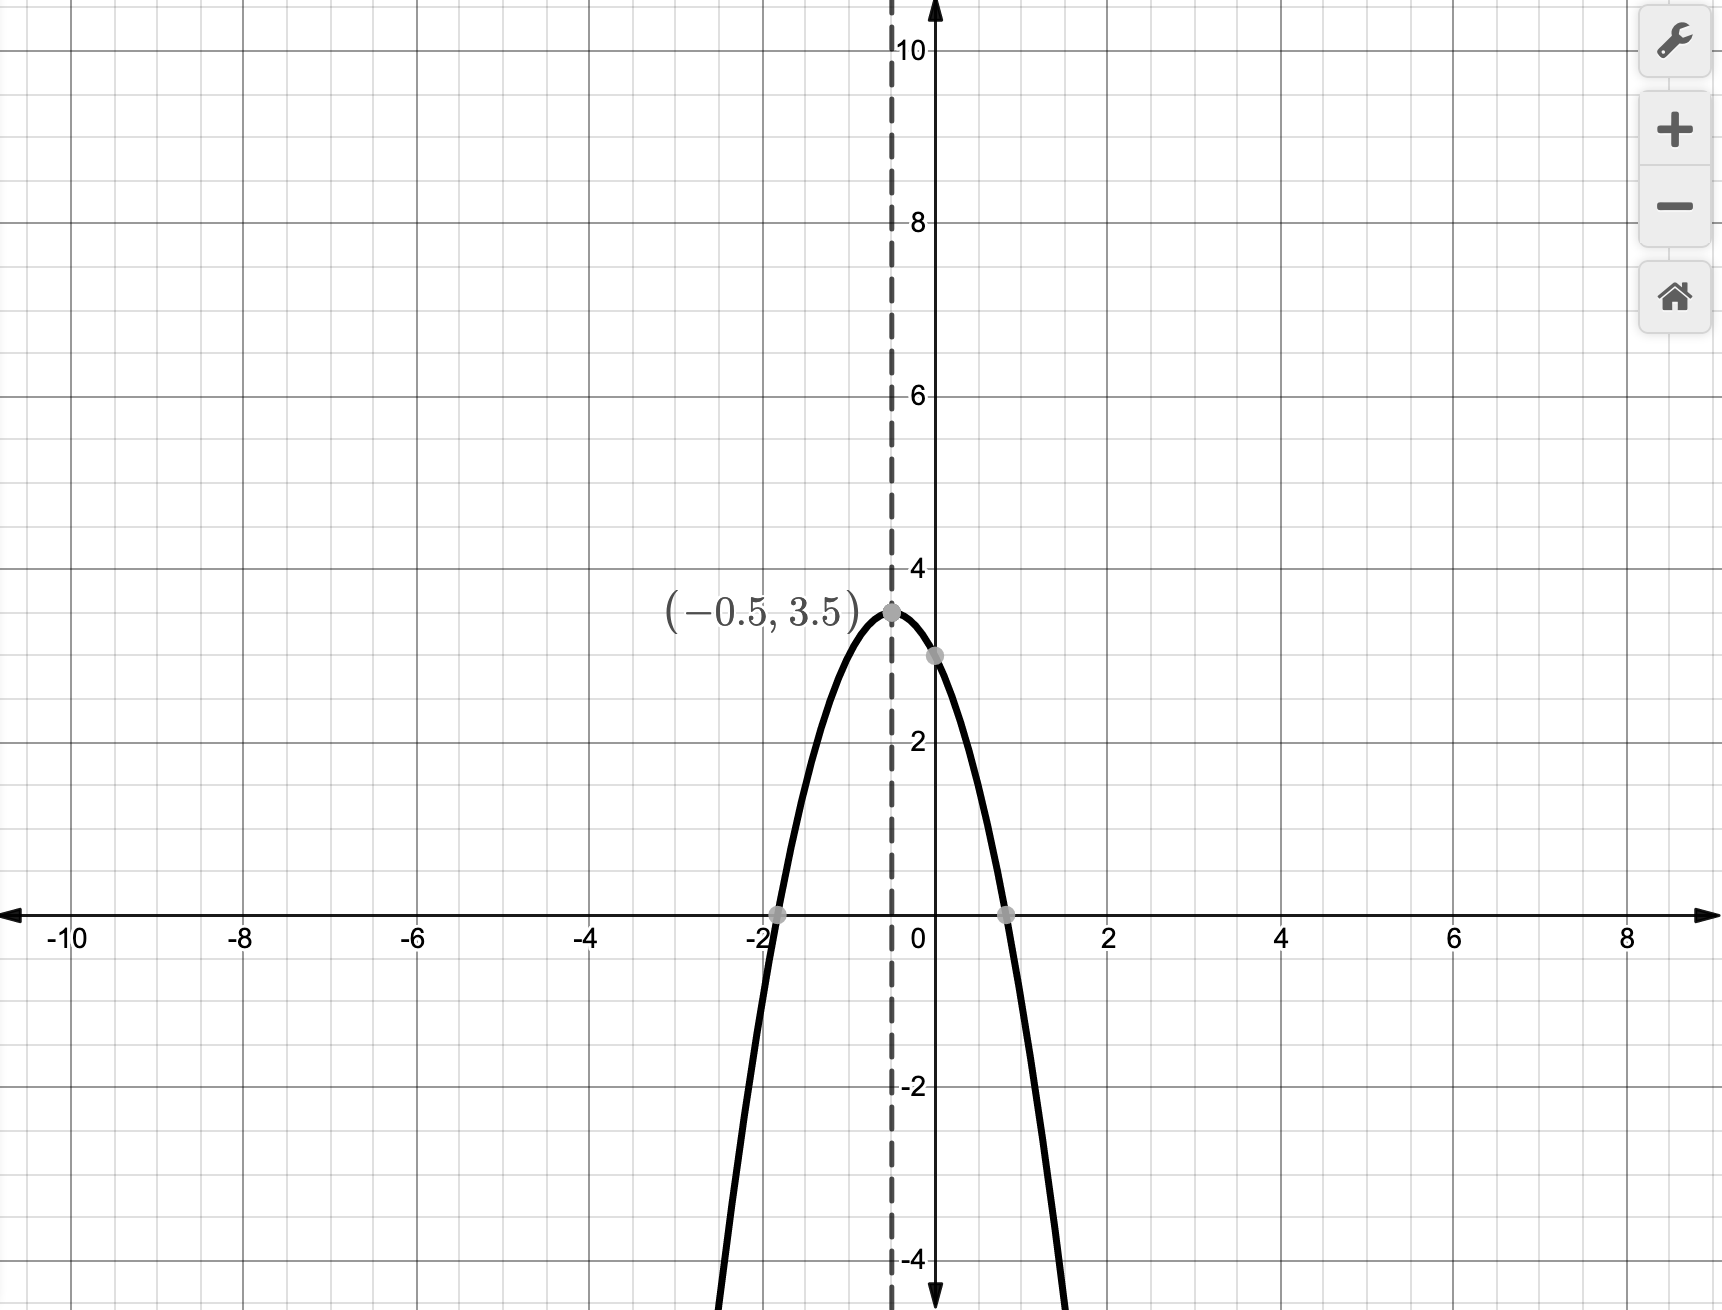
\includegraphics[scale=0.25]{3_3_3.png}
			\end{center}
	\end{enumerate}
\end{frame}

\begin{frame}
	\frametitle{Example}
	\begin{enumerate}
		\item[]<1-> Find the vertex, the axis of symmetry, and the maximum or minimum value of
		\item[]<2->\[ g(x)=\frac{x^{2}}{2}-4x+8. \]
		\item[]<3-> \textsc{Solution:}
		\item[]<4-> The vertex is $V=\left( -\frac{-4}{2(1/2)}, f \left( -\frac{-4}{2(1/2))} \right)\right)=\left( 4, 0 \right)$.
		\item[]<5-> The axis of symmetry is $x=4$.
		\item[]<6-> The function has a minimum of $y=0$.
	\end{enumerate}
\end{frame}

\begin{frame}
	\frametitle{Example (cont.)}
	\begin{enumerate}
		\item[]<1-> The graph of the function is
		\item[]<2->\begin{center}
				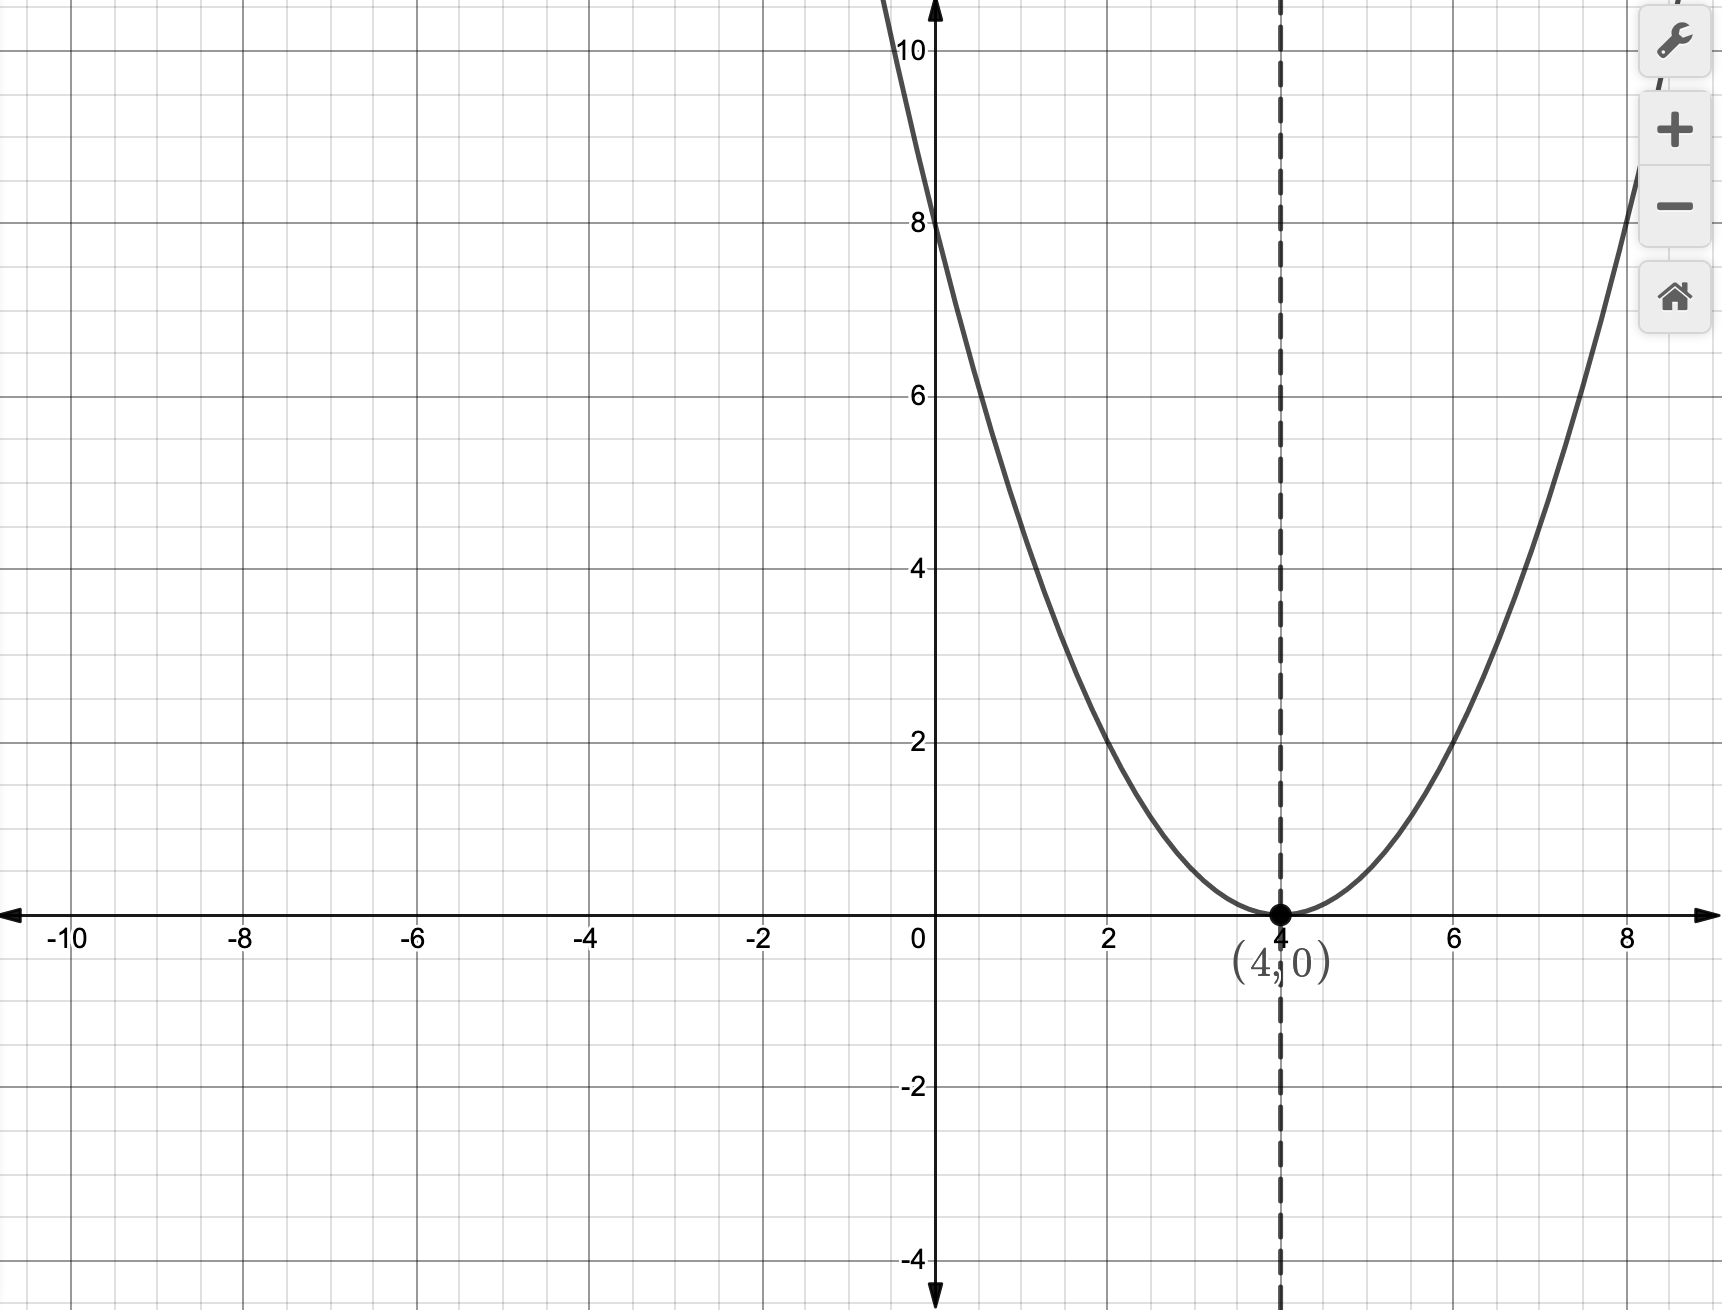
\includegraphics[scale=0.25]{3_3_4.png}
			\end{center}
	\end{enumerate}
\end{frame}

\begin{frame}
	\frametitle{Example}
	\begin{enumerate}
		\item[]<1-> Find the vertex, the axis of symmetry, and the maximum or minimum value of
		\item[]<2->\[ f(x)=x^{2}-9x+18. \]
		\item[]<3-> \textsc{Solution:}
		\item[]<4-> The vertex is $V=\left( -\frac{-9}{2(1)}, f \left( -\frac{-9}{2(1))} \right)\right)=\left( \frac{9}{2}, -\frac{9}{4}\right)$.
		\item[]<5-> The axis of symmetry is $x=\frac{9}{2}$.
		\item[]<6-> The function has a minimum of $y=-\frac{9}{4}$.
	\end{enumerate}
\end{frame}

\begin{frame}
	\frametitle{Example (cont.)}
	\begin{enumerate}
		\item[]<1-> The graph of the function is
		\item[]<2->\begin{center}
				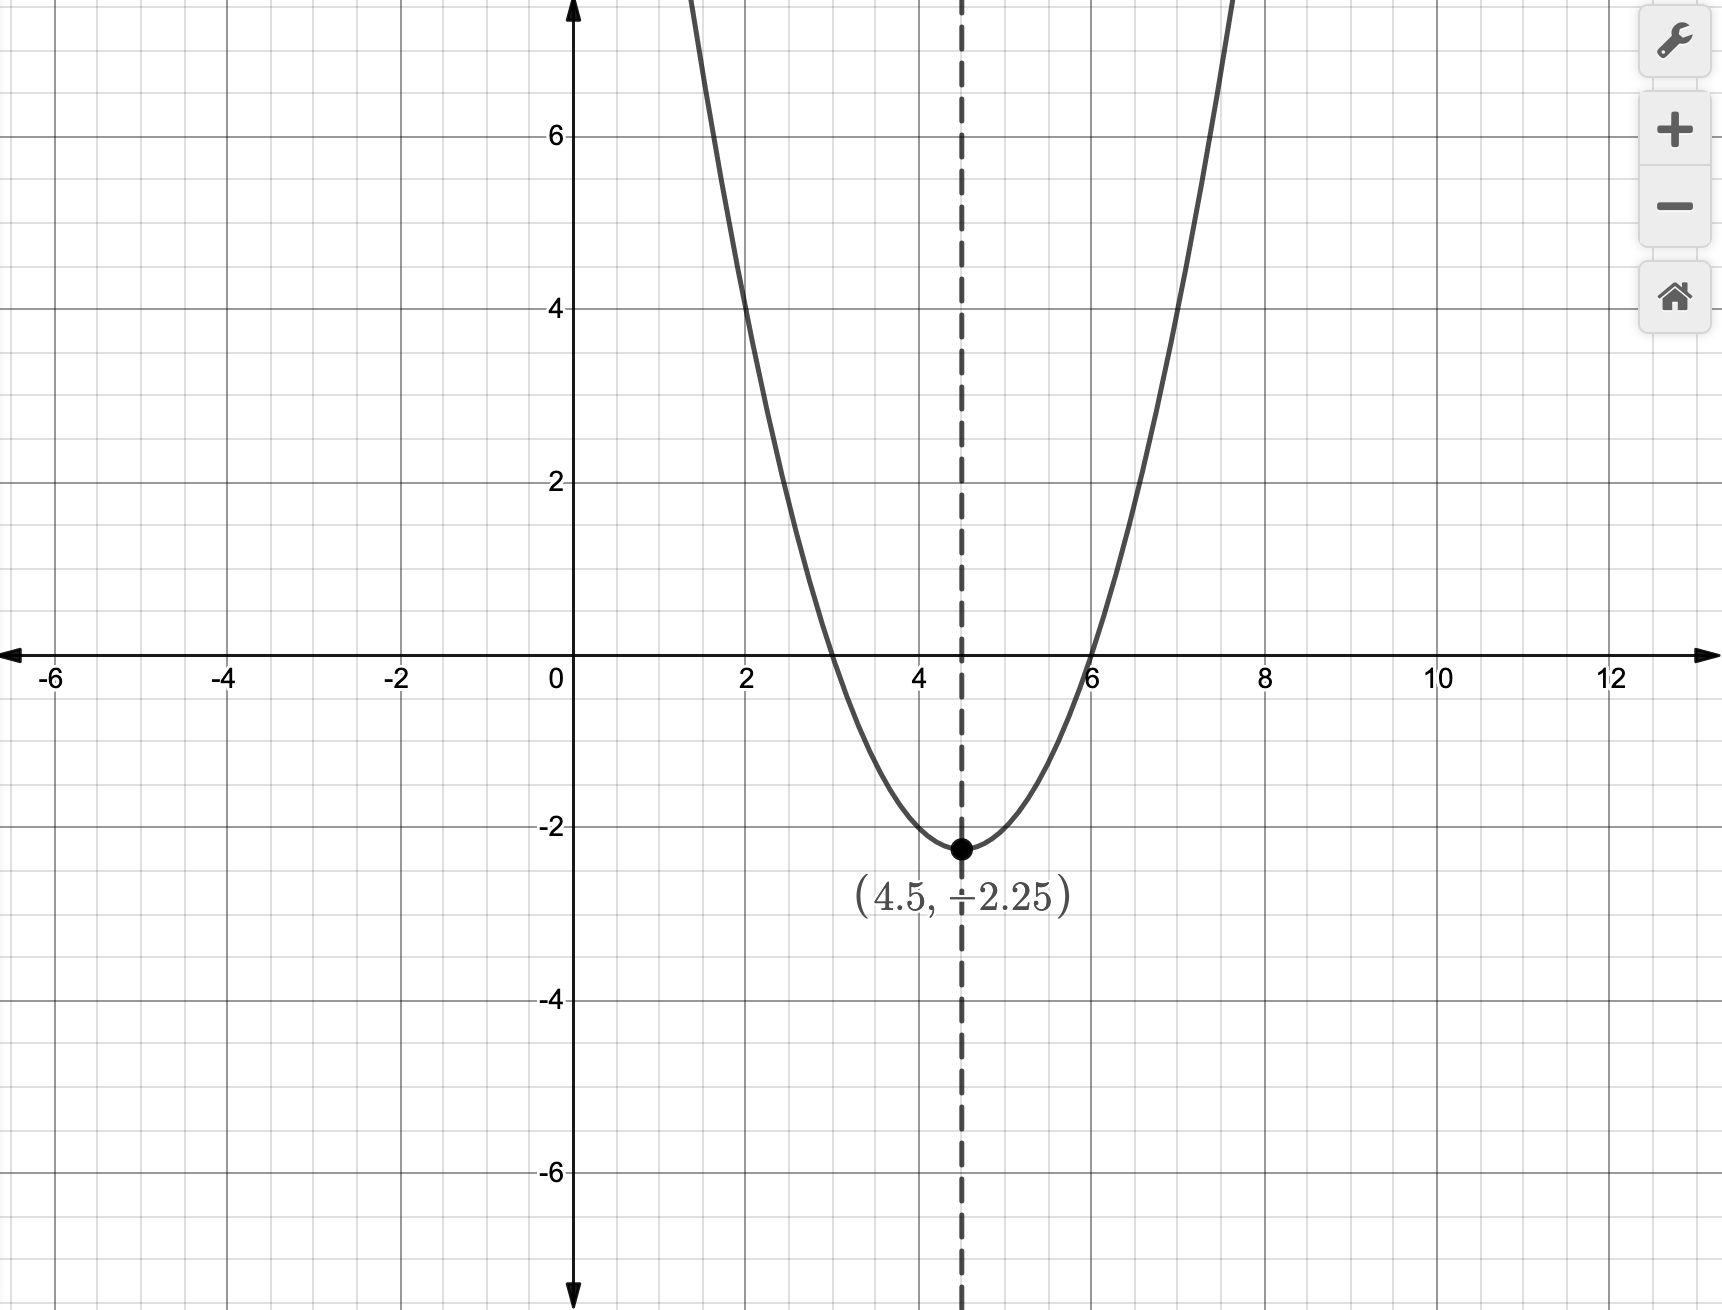
\includegraphics[scale=0.25]{3_3_6.png}
			\end{center}
	\end{enumerate}
\end{frame}

\begin{frame}
	\frametitle{Example}
	\begin{enumerate}
		\item[]<1-> Find the vertex, the axis of symmetry, and the maximum or minimum value of
		\item[]<2->\[ f(x)=-x^{2}-4x-5. \]
		\item[]<3-> \textsc{Solution:}
		\item[]<4-> The vertex is $V=\left( -\frac{-4}{2(-1)}, f \left( -\frac{-4}{2(-1))} \right)\right)=\left( -2,  -1 \right)$.
		\item[]<5-> The axis of symmetry is $x=-2$.
		\item[]<6-> The function has a maximum of $y=-1$.
	\end{enumerate}
\end{frame}

\begin{frame}
	\frametitle{Example (cont.)}
	\begin{enumerate}
		\item[]<1-> The graph of the function is
		\item[]<2->\begin{center}
				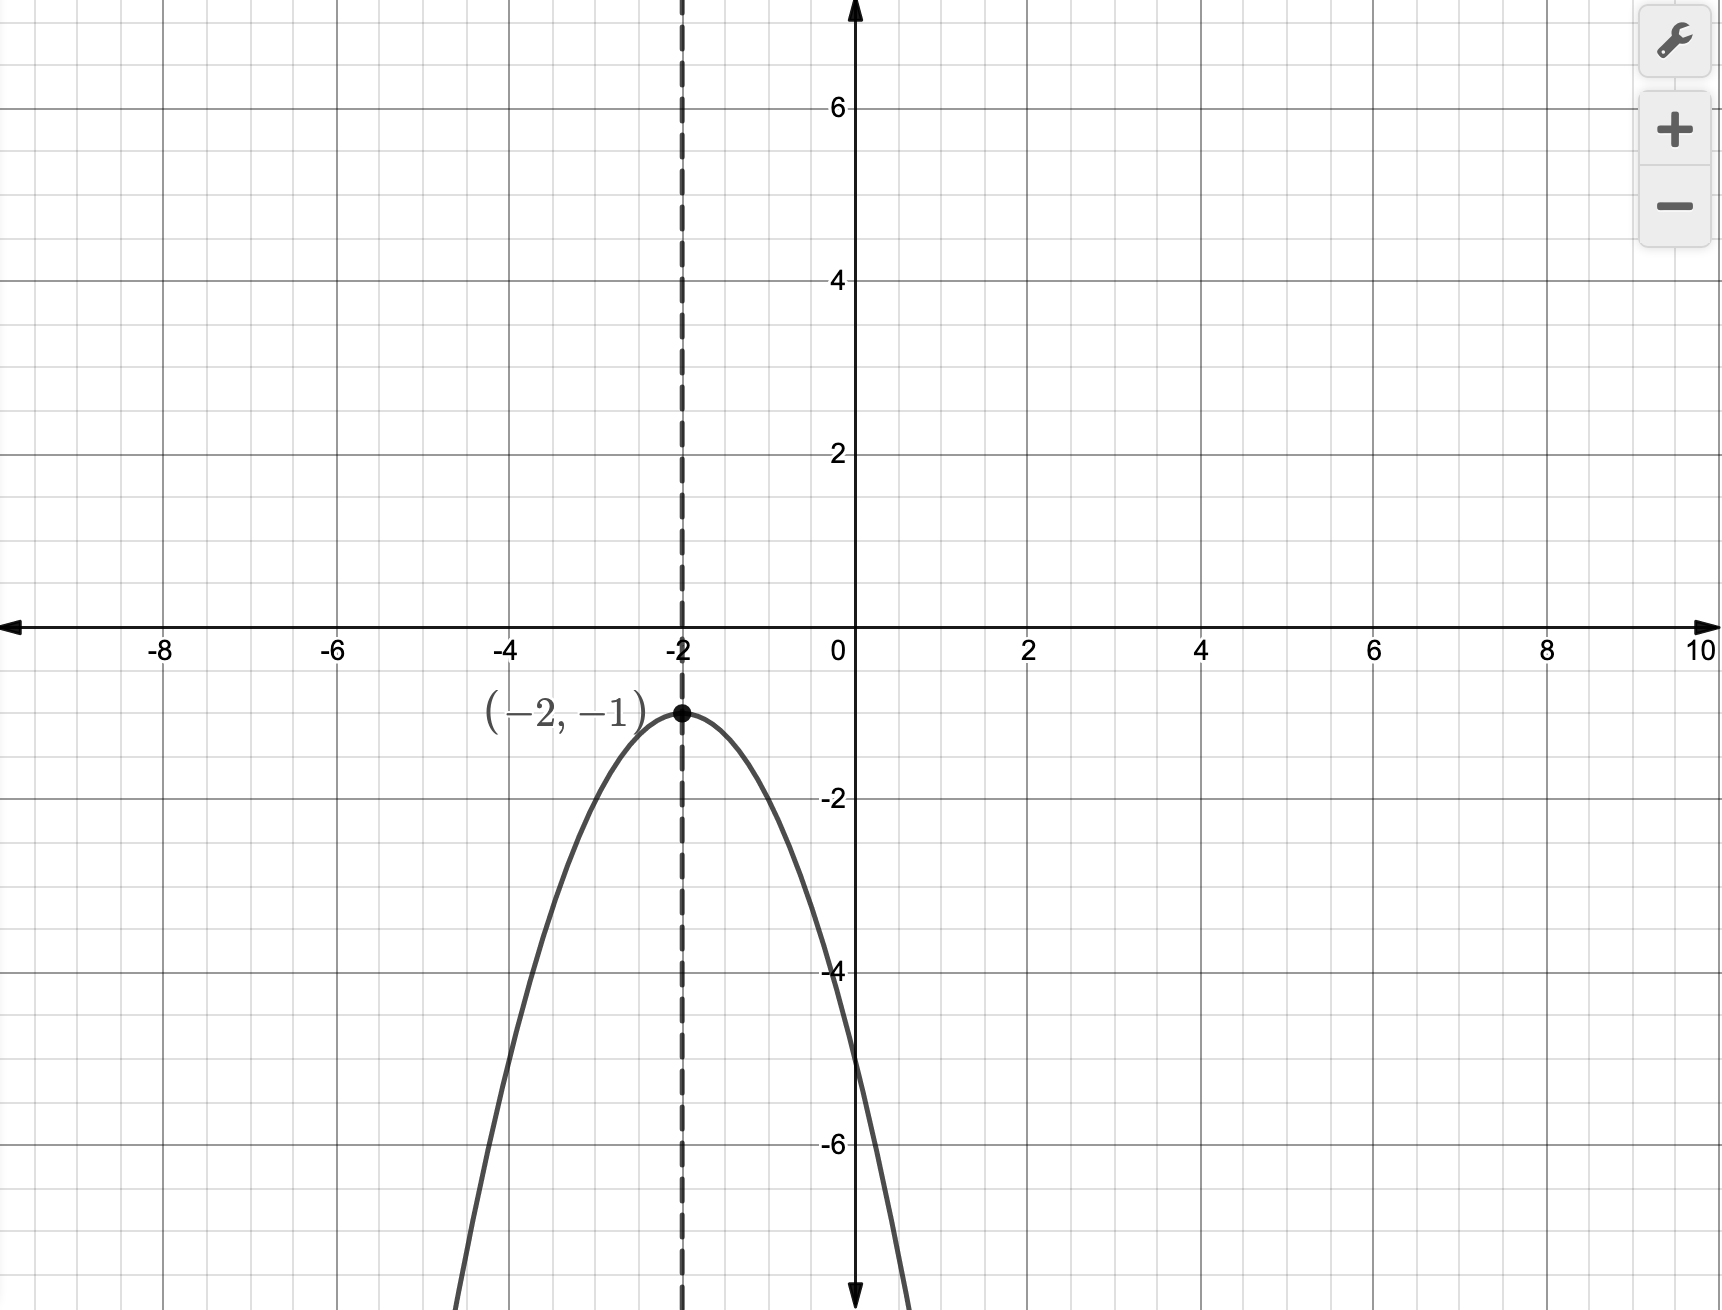
\includegraphics[scale=0.25]{3_3_7.png}
			\end{center}
	\end{enumerate}
\end{frame}

\begin{frame}
	\frametitle{Example}
	\begin{enumerate}
		\item[]<1->For the function
		\[
			f(x)=-x^{2}+14x-47;
		\]
		\item[]<2-> (a) find the vertex:
		\item[]<3-> \textsc{Solution:}
		\item[]<4->\[ \Rightarrow V=\left(-\frac{14}{2(-1)}, f \left( -\frac{14}{2(-1)} \right)  \right) \]
		\item[]<5-> \[ \Rightarrow V= \left( 7, 2 \right) \]
	\end{enumerate}
\end{frame}

\begin{frame}
	\frametitle{Example (cont.)}
	\begin{enumerate}
		\item[]<1-> (b) determine whether there is a maximum or minimum value, and find that value:
		\item[]<2-> \textsc{Solution:}
		\item[]<3-> Given that $a=-1<0$, there is a maximum value for $f(x)$.
		\item[]<4-> The value is the $y-$value of the vertex, namely
		\item[]<5-> \[ y=2. \]
	\end{enumerate}
\end{frame}

\begin{frame}
	\frametitle{Example (cont.)}
	\begin{enumerate}
		\item[]<1-> (c) on what intervals is the function increasing and/or decreasing:
		\item[]<2-> \textsc{Solution:}
		\item[]<3-> $f(x)$ is increasing on \[ \left( -\infty, 7\right);  \]
		\item[]<4-> $f(x)$ is decreasing on
		\[
			(7, \infty).
		\]
	\end{enumerate}
\end{frame}

\begin{frame}
	\frametitle{Example}
	\begin{enumerate}
		\item[]<1-> Graph the function
		\[
			f(x)=-(x-3)^{2}
		\]
		\item[]<2-> \textsc{Solution:}
		\item[]<3-> We note that the vertex $V$ is
		\item[]<4-> \[ V=(3,0), \]
		\item[]<5-> with $a=-1<0$, which implies that the graph opens downwards.
	\end{enumerate}
\end{frame}

\begin{frame}
	\frametitle{Example (cont.)}
	\begin{enumerate}
		\item[]<1-> The only graph which meets the above criteria is
		\item[]<2->
		\begin{figure}
			\begin{center}
				\caption{D.}
				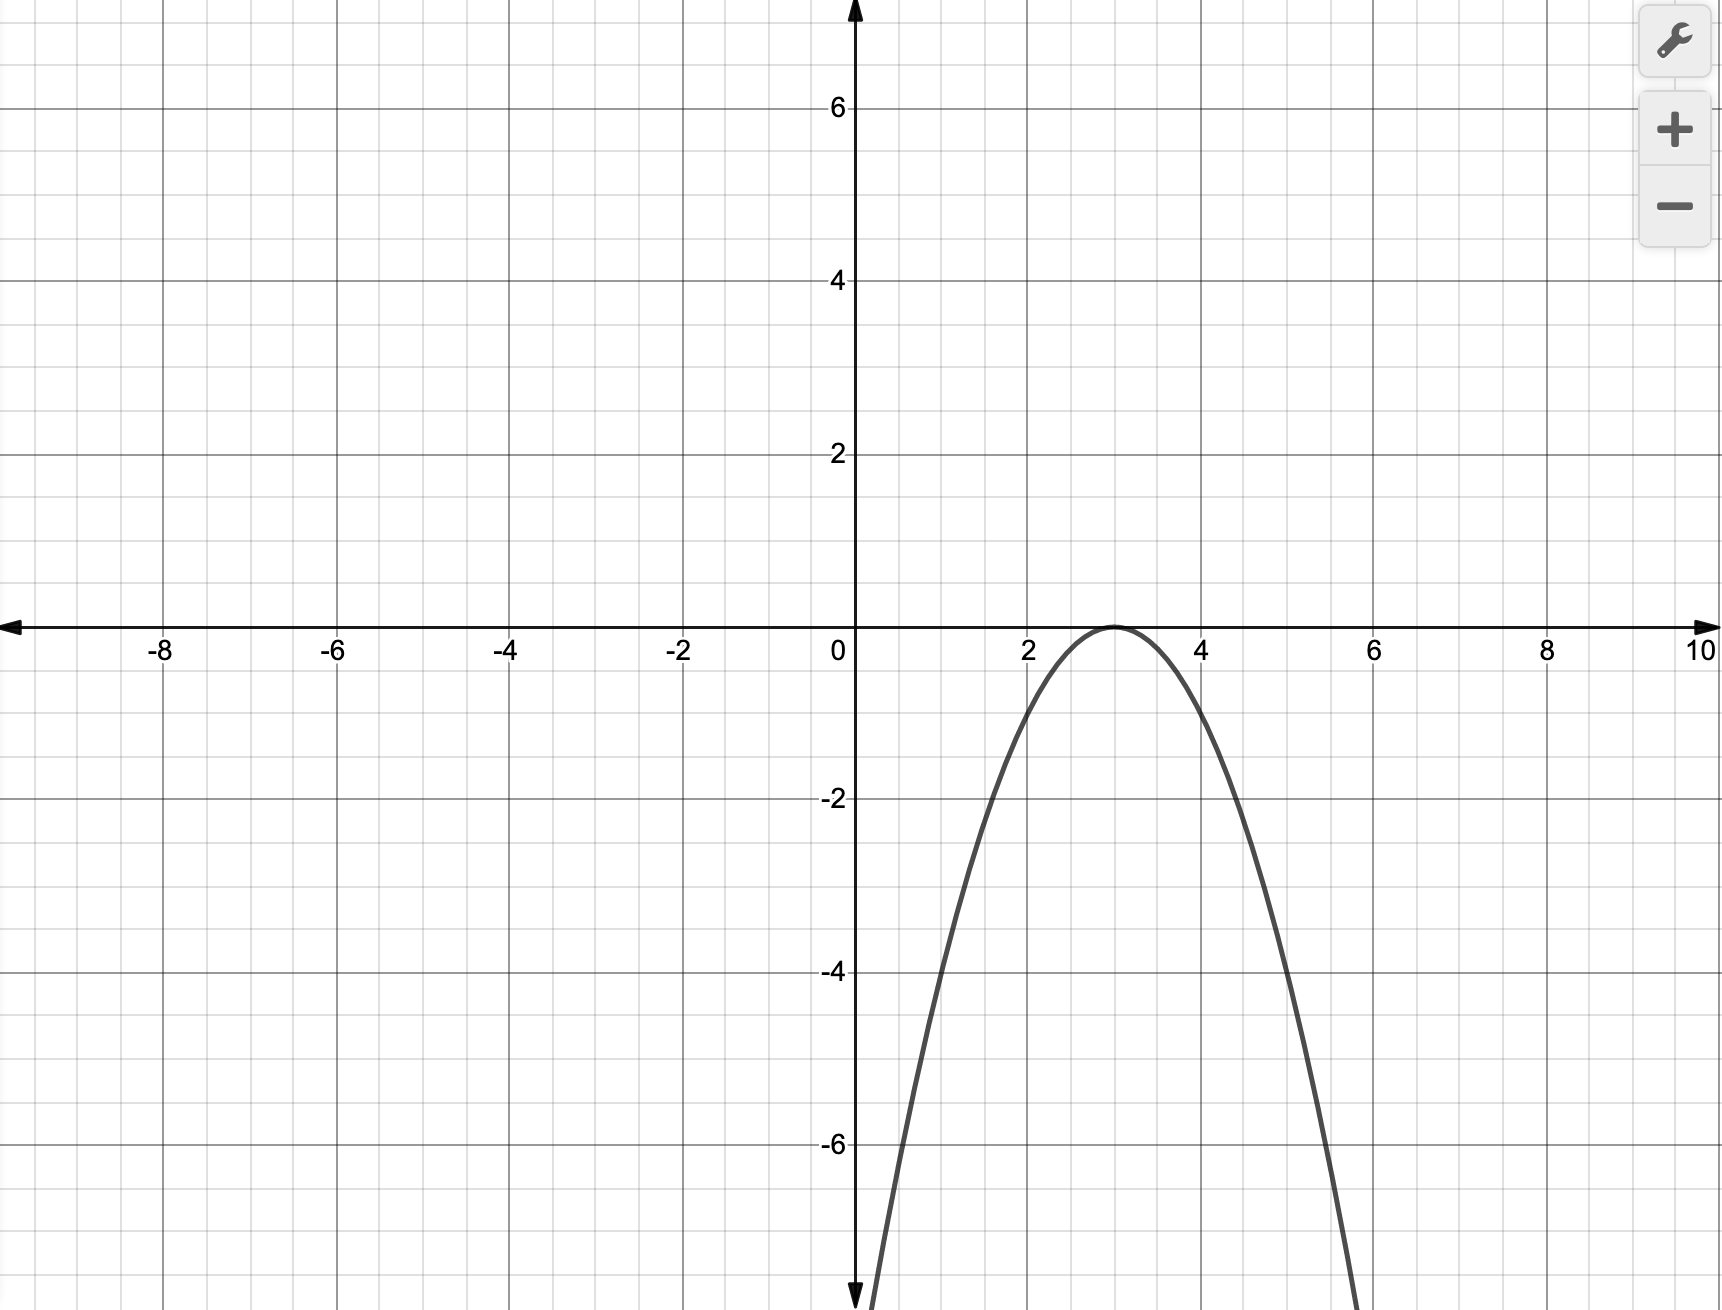
\includegraphics[scale=0.2]{3_3_8.png}
			\end{center}
		\end{figure}
	\end{enumerate}
\end{frame}

\begin{frame}
	\frametitle{Example}
	\begin{enumerate}
		\item[]<1-> Graph the function
		\[
			f(x)=4(x+9)^{2}+1
		\]
		\item[]<2-> \textsc{Solution:}
		\item[]<3-> We note that the vertex $V$ is
		\item[]<4-> \[ V=(-9, 1), \]
		\item[]<5-> with $a=4>0$, which implies that the graph opens upwards.
	\end{enumerate}
\end{frame}

\begin{frame}
	\frametitle{Example (cont.)}
	\begin{enumerate}
		\item[]<1-> The only graph which meets the above criteria is
		\item[]<2->
		\begin{figure}
			\begin{center}
				\caption{D.}
				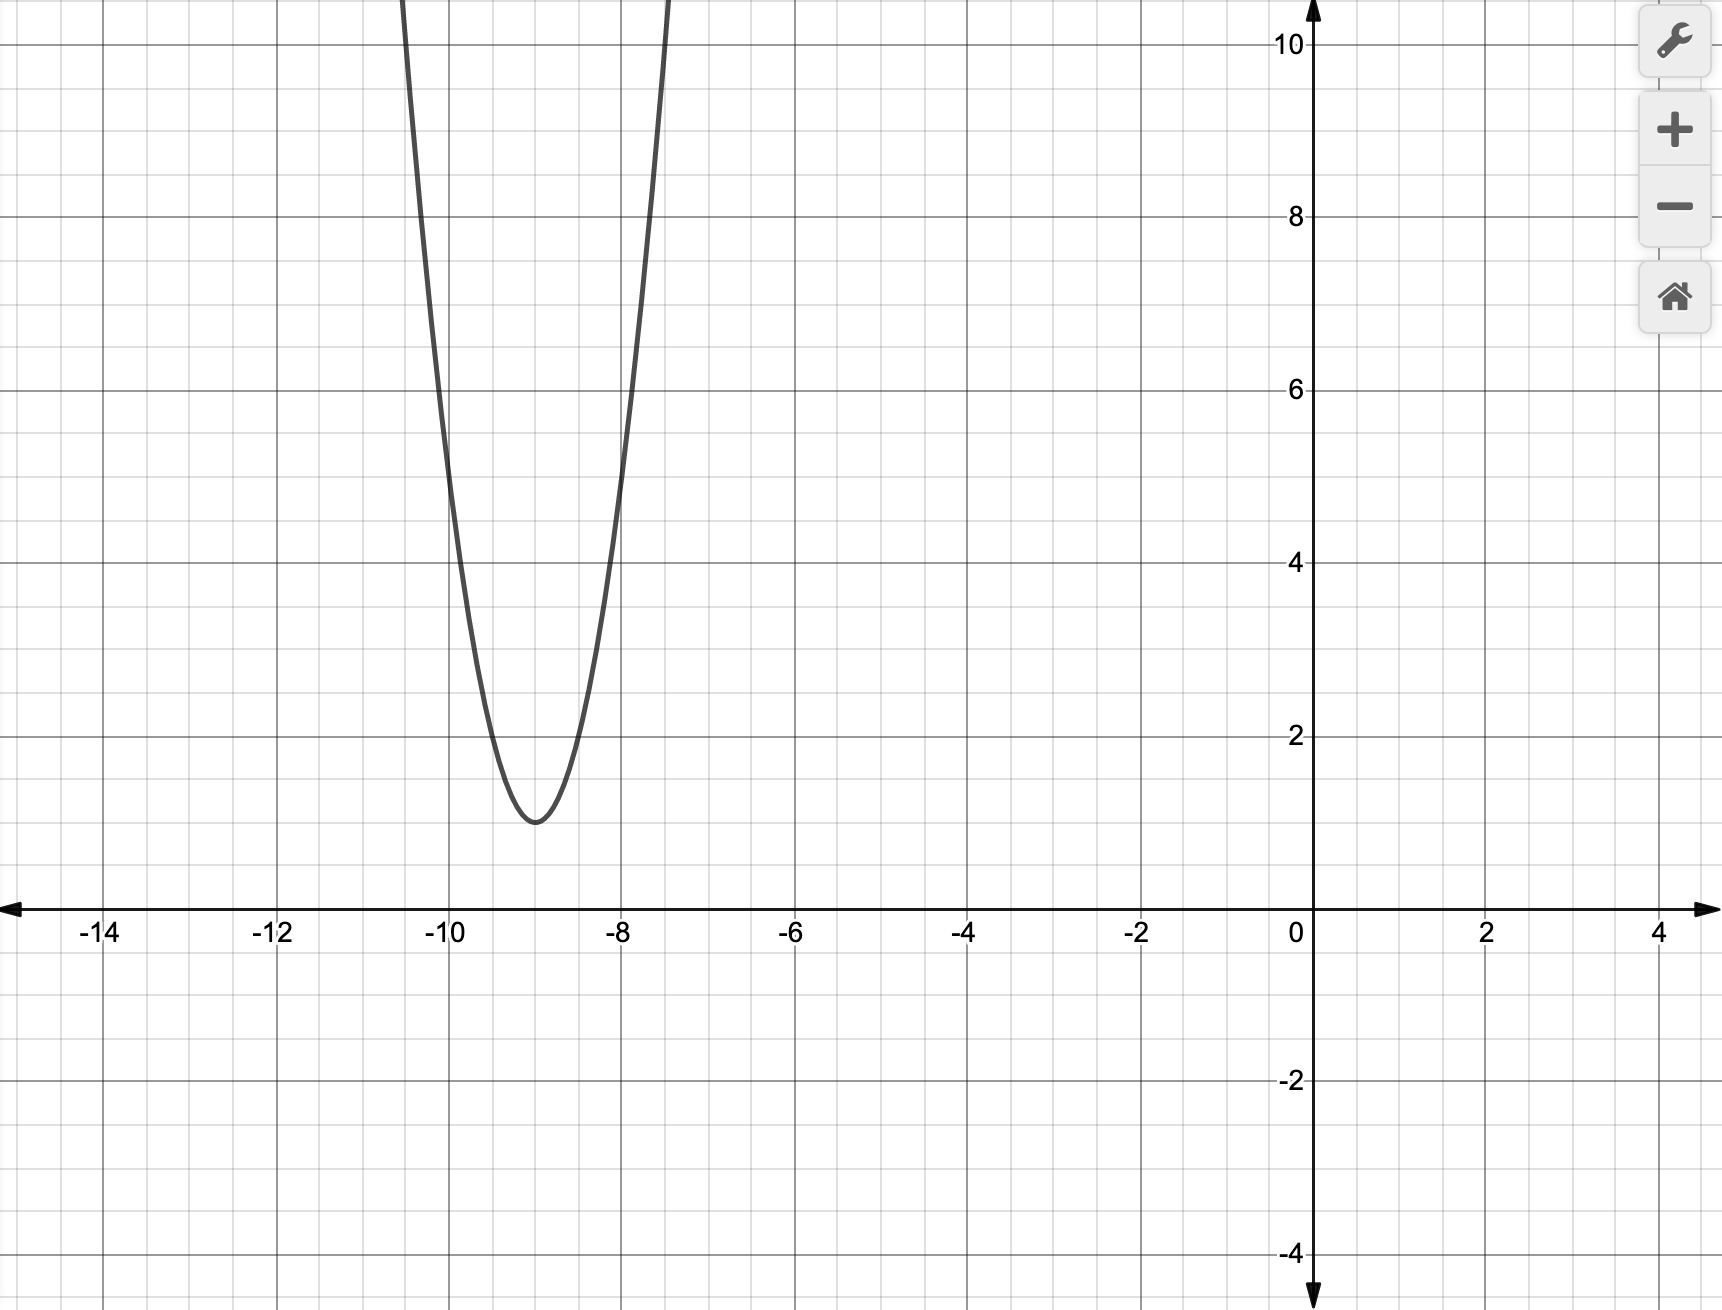
\includegraphics[scale=0.2]{3_3_9.png}
			\end{center}
		\end{figure}
	\end{enumerate}
\end{frame}

\begin{frame}
	\frametitle{Example}
	\begin{enumerate}
		\item[]<1-> Given the function
		\[
			f(x)=x^{2}-10x+24
		\]
		\item[]<2-> (a) find the vertex,
		\item[]<3-> \textsc{Solution:}
		\item[]<4-> \[ V= \left(-\frac{-10}{2(1)}, f \left(-\frac{-10}{2(1)} \right) \right) \]
		\item[]<5-> \[ \Rightarrow V=\left( 5, -1 \right) \]
		\item[]<6-> (b) determine whether there is a maximum or a minimum value,
	\end{enumerate}
\end{frame}

\begin{frame}
	\frametitle{Example (cont.)}
	\begin{enumerate}
		\item[]<1->\textsc{Solution:}
		\item[]<2-> Since $a=1>0$, the graph of $f(x)$ opens upwards, and
		\item[]<3->there is a minimum value, which is the $y-$value of the vertex, namely
		\item[]<4-> \[ y=-1.\]
		\item[]<5-> (c) find the range,
		\item[]<6-> \textsc{Solution:}
		\item[]<7-> The range comprises the possible $y-$values of $f(x)$, and so is
		\item[]<8-> \[ [-1, \infty).  \]
	\end{enumerate}
\end{frame}

\begin{frame}
	\frametitle{Example (cont.)}
	\begin{enumerate}
		\item[]<1-> (d) find the intervals on which the function is increasing and the intervals on which the function is decreasing,
		\item[]<2-> \textsc{Solution:}
		\item[]<3-> The function $f(x)$ is increasing on the interval
		\item[]<4-> \[ (5, \infty),\]
		\item[]<5-> and the function $f(x)$ is decreasing on the interval
		\item[]<6-> \[ (-\infty, 5). \]
	\end{enumerate}
\end{frame}

\begin{frame}
	\frametitle{Example}
	\begin{enumerate}
		\item[]<1-> Use the graph below to find the vertex, the axis of symmetry, and the maximum or minimum of the function.
		\item[]<2->
			\begin{center}
				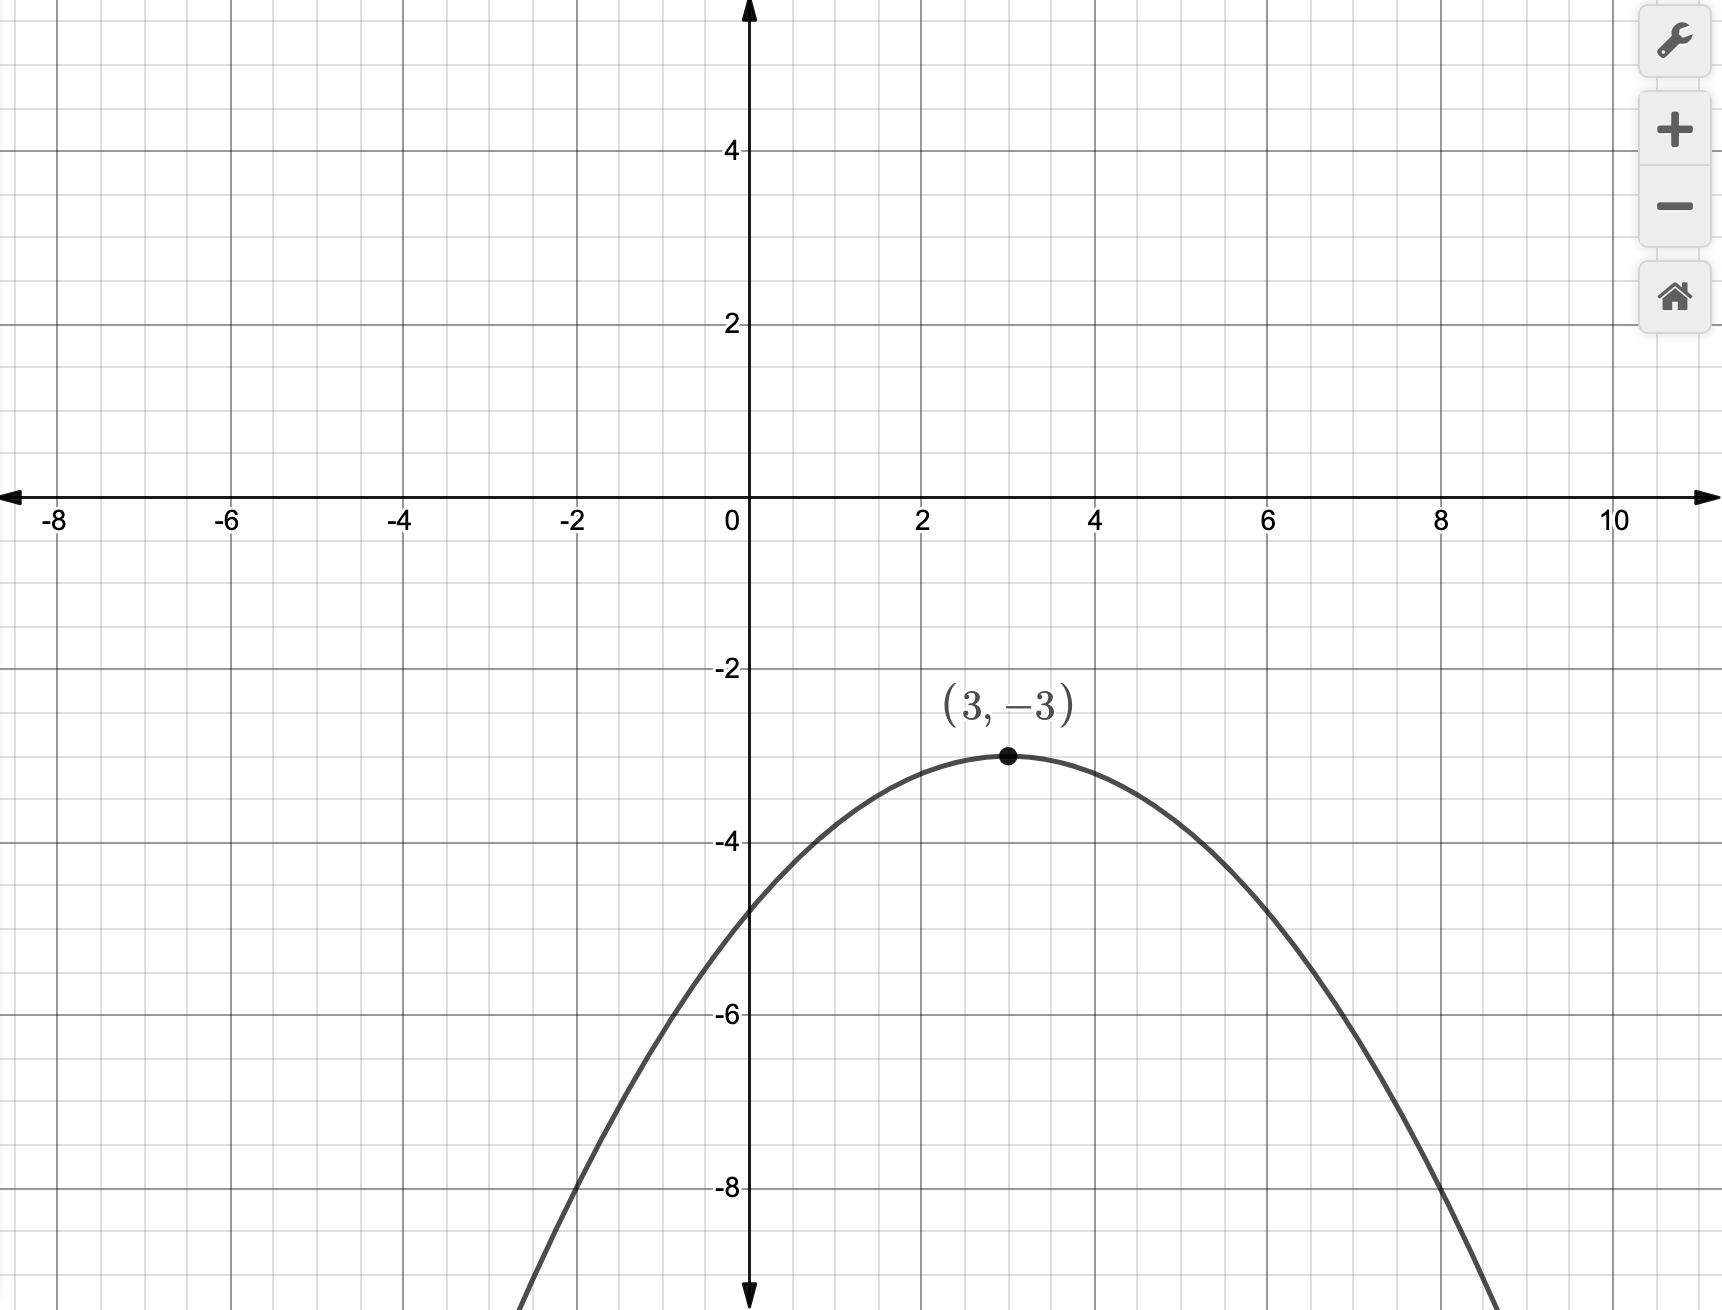
\includegraphics[scale=0.2]{3_3_10.png}
			\end{center}
	\end{enumerate}
\end{frame}

\begin{frame}
	\frametitle{Example (cont.)}
	\begin{enumerate}
		\item[]<1-> \textsc{Solution:}
		\item[]<2-> The vertex $V$ is
			\[
				V=(3,-3).
			\]
		\item[]<3-> The axis of symmetry is
		\[
			x=3.
		\]
		\item[]<4-> The function has a maximum value of
		\[
			y=-3.
		\]
	\end{enumerate}
\end{frame}

\begin{frame}
	\frametitle{Example}
	\begin{enumerate}
		\item[]<1-> Find the vertex of the parabola
			\[
				f(x)=-2x^{2}-20x-53.
			\]
		\item[]<2-> \textsc{Solution:}
		\item[]<3-> \[ V= \left( -\frac{-20}{2(-2)}, f \left( -\frac{-20}{2(-2)}\right) \right) \]
		\item[]<4-> \[ \Rightarrow V= (-5,-3) ~~(B.) \]
	\end{enumerate}
\end{frame}

\begin{frame}
	\frametitle{Example}
	\begin{enumerate}
		\item[]<1-> Find the vertex of the parabola
		\[
			f(x)=-x^{2}+7x-5.
		\]
		\item[]<2-> \textsc{Solution:}
		\item[]<3-> \[ V= \left( -\frac{7}{2(-1)}, f \left(  -\frac{-7}{2(-1)}\right) \right) \]
		\item[]<4-> \[ \Rightarrow V=\left( \frac{7}{2}, \frac{29}{4} \right)~~(C.) \]
	\end{enumerate}
\end{frame}

\begin{frame}
	\frametitle{Example}
	\begin{enumerate}
		\item[]<1-> Find the axis of symmetry of the given function
		\[
			f(x)=-3x^{2}+6x.
		\]
		\item[]<2-> \textsc{Solution:}
		\item[]<3-> We need only find
		\[
			-\frac{b}{2a}.
		\]
		\item[]<4->
		\[
			\Rightarrow x=-\frac{6}{2(-3)}=1.~~(B.)
		\]
	\end{enumerate}
\end{frame}

\begin{frame}
	\frametitle{Example}
	\begin{enumerate}
		\item[]<1-> Find the axis of symmetry of the given function
		\[
			f(x)=4x^{2}-16x+20
		\]
		\item[]<2-> \textsc{Solution:}
		\item[]<3-> We need only find
		\[
			-\frac{b}{2a}.
		\]
		\item[]<4->
		\[
			\Rightarrow x=-\frac{-16}{2(4)}=2.~~(C.)
		\]
	\end{enumerate}
\end{frame}

\begin{frame}
	\frametitle{Example}
	\begin{enumerate}
		\item[]<1-> Determine whether there is a maximum or minimum value for the given function, and find that value:
		\item[]<2-> \[ f(x)=x^{2}+4x-5. \]
		\item[]<3-> \textsc{Solution:}
		\item[]<4-> Since $a=1>0$, there is a minimum value of $f(x)$.
		\item[]<5-> The minimum value is the $y-$value of the vertex. which is
		\item[]<6-> \[ f(x)=-9~~(D.)\]
	\end{enumerate}
\end{frame}

\begin{frame}
	\frametitle{Example}
	\begin{enumerate}
		\item[]<1-> Determine whether there is a maximum or minimum value for the given function, and find that value:
		\item[]<2-> \[ f(x)=-2x^{2}-4x-8. \]
		\item[]<3-> \textsc{Solution:}
		\item[]<4-> Since $a=-2<0$, there is a maximum value of $f(x)$.
		\item[]<5-> The maximum value is the $y-$value of the vertex. which is
		\item[]<6-> \[ f(x)=-6~~(D.)\]
	\end{enumerate}
\end{frame}

\section{$\S 3.4$: Solving Rational Equations \& Radical Equations}

\begin{frame}
	\frametitle{Example}
	\begin{enumerate}
		\item[]<1-> Solve
		\[
			\frac{x+6}{4}-\frac{x-3}{5}=3
		\]
		\item[]<2-> \textsc{Solution:}
		\item[]<3-> \[ \text{\textsc{lcd}}=20 \Rightarrow 20 \left( \frac{x+6}{4}\right)-20\left(\frac{x-3}{5}\right)=20(3)\]
		\item[]<4-> \[ \Rightarrow 5(x+6)-4(x-3)=60 \]
		\item[]<5-> \[ \Rightarrow 5x+30-4x+12=60 \]
		\item[]<6-> \[ \Rightarrow x+42=60  \]
		\item[]<7-> \[ \Rightarrow x=18.  \]
	\end{enumerate}
\end{frame}

\begin{frame}
	\frametitle{Example}
	\begin{enumerate}
		\item[]<1->Solve
		\[
			\frac{x-8}{3}-\frac{x-3}{2}=0.
		\]
		\item[]<2->\textsc{Solution:}
		\item[]<3->
		\begin{align*}
			\text{\textsc{lcd}}=3(2)=6 & \Rightarrow 6 \cdot \frac{x-8}{3}- 6 \cdot \frac{x-3}{2}= 6 \cdot 0.  \\
			& \Rightarrow 2(x-8)-3(x-3)=0 \\
			& \Rightarrow 2x-16-3x+9=0 \\
			& \Rightarrow -x-7=0 \\
			& \Rightarrow x=-7.
		\end{align*}
	\end{enumerate}
\end{frame}

\begin{frame}
	\frametitle{Example}
	\begin{enumerate}
		\item[]<1->Solve
		\[
			\frac{2}{x+4}=\frac{4}{x}
		\]
		\item[]<2-> \textsc{Solution:}
		\item[]<3->
		\begin{align*}
			\text{\textsc{lcd}}= & \Rightarrow x(x+4) \left( \frac{2}{x+4}\right)=x(x+4) \left( \frac{4}{x} \right) \\
			& \Rightarrow 2x=4(x+4) \\
			& \Rightarrow 2x=4x+16 \\
			& \Rightarrow -2x=16 \\
			& \Rightarrow x=-8.
		\end{align*}
	\end{enumerate}
\end{frame}

\begin{frame}
	\frametitle{Example}
	\begin{enumerate}
		\item[]<1->Solve \[ \frac{x^{2}}{x-3}=\frac{9}{x-3}. \]
		\item[]<2-> \textsc{Solution:}
		\item[]<3-> \[ \text{\textsc{lcd}}=x-3 \Rightarrow (x-3) \left( \frac{x^{2}}{x-3} \right)=(x-3) \left( \frac{9}{x-3}\right)\]
		\item[]<4-> \[\Rightarrow  x^{2}=9 \]
		\item[]<5->\[ \Rightarrow x=\pm 3 \]
		\item[]<6-> But $x=3$ gives us $\frac{3^{2}}{0}=\frac{9}{0}$, which does not exist.
		\item[]<7-> \[ \Rightarrow x=-3. \]
	\end{enumerate}
\end{frame}

\begin{frame}
	\frametitle{Example}
	\begin{enumerate}
		\item[]<1->Solve
		\[
			\frac{y^{2}}{y+7}=\frac{49}{y+7}.
		\]
		\item[]<2-> \textsc{Solution:}
		\item[]<3->
		\begin{align*}
			\text{\textsc{lcd}}=7 & \Rightarrow y+7 \left( \frac{y^{2}}{y+7}\right)=(y+7) \left( \frac{49}{y+7}\right)  \\
			& \Rightarrow y^{2}=49 \\
			& \Rightarrow y= \pm 7 \\
			& \Rightarrow \cancel{y=-7}, y=7.
		\end{align*}
	\end{enumerate}
\end{frame}

\begin{frame}
	\frametitle{Example}
	\begin{enumerate}
		\item[]<1->Solve
		\[
			\frac{x+9}{3}-\frac{x-12}{4}=3
		\]
		\item[]<2-> \textsc{Solution:}
		\item[]<3->
		\begin{align*}
			\text{\textsc{lcd}}=12 & \Rightarrow 12 \left( \frac{x+9}{3} \right)-12 \left( \frac{x-12}{4} \right)=12(3)  \\
			& \Rightarrow 4(x+9)-3(x-12)=36 \\
			& \Rightarrow 4x-36-3x+36=36 \\
			& \Rightarrow x=-36.
		\end{align*}
	\end{enumerate}
\end{frame}

\begin{frame}
	\frametitle{Example}
	\begin{enumerate}
		\item[]<1->Solve
		\[
			\frac{4}{x+2}=\frac{6}{x}
		\]
		\item[]<2-> \textsc{Solution:}
		\item[]<3->
		\begin{align*}
			\text{\textsc{lcd}}=x(x+2) & \Rightarrow x(x+2) \left( \frac{4}{x+2} \right)=x(x+2) \left( \frac{6}{x} \right) \\
			& \Rightarrow 4x=6(x+2) \\
			& \Rightarrow 4x=6x+12 \\
			& \Rightarrow -2x=12 \\
			& \Rightarrow x=-6.
		\end{align*}
	\end{enumerate}
\end{frame}

\begin{frame}
	\frametitle{Example}
	\begin{enumerate}
		\item[]<1->Solve
		\[
			\frac{2}{7}+\frac{1}{4}=\frac{1}{x}.
		\]
		\item[]<2-> \textsc{Solution:}
		\item[]<3-> \[ \text{\textsc{lcd}}=28x \Rightarrow 28x \left( \frac{2}{7} \right)+28x\left(\frac{1}{4} \right) =28x \left( \frac{1}{x} \right) \]
		\item[]<4-> \[ \Rightarrow 8x+7x=28 \]
		\item[]<5-> \[ \Rightarrow 15x=28 \]
		\item[]<6-> \[ \Rightarrow x=\frac{28}{15}. \]
	\end{enumerate}
\end{frame}

\begin{frame}
	\frametitle{Example}
	\begin{enumerate}
		\item[]<1-> Solve
		\[
			\frac{x+9}{3}-\frac{x-12}{4}=3.
		\]
		\item[]<2-> \textsc{Solution:}
		\item[]<3-> \[ \text{\textsc{lcd}}=3(4)=12 \Rightarrow 12 \left( \frac{x+9}{3} \right)-12\left( \frac{x-12}{4} \right)=12(3)  \]
		\item[]<4-> \[ \Rightarrow 4(x+9)-3(x-12)=36\]
		\item[]<5-> \[ \Rightarrow 4x+36-3x+36=36 \]
		\item[]<6-> \[ \Rightarrow x=-36. \]
	\end{enumerate}
\end{frame}

\begin{frame}
	\frametitle{Example}
	\begin{enumerate}
		\item[]<1-> Solve
		\[
			\frac{7}{p}+p=-8.
		\]
		\item[]<2-> \textsc{Solution:}
		\item[]<3-> \[ \text{\textsc{lcd}}=p \Rightarrow p \left( \frac{7}{p} \right) +p(p)=-8p \]
		\item[]<4-> \[ \Rightarrow 7+p^{2}=-8p \]
		\item[]<5-> \[ \Rightarrow p^{2}+8p+7=0 \]
		\item[]<6-> \[ \Rightarrow (p+7)(p+1)=0 \]
	\end{enumerate}
\end{frame}

\begin{frame}
	\frametitle{Example (cont.}
	\begin{enumerate}
		\item[]<1-> \[ \Rightarrow p+7=0, p+1=0 \]
		\item[]<2-> \[\Rightarrow p=-7, p=-1. \]
	\end{enumerate}
\end{frame}

\begin{frame}
	\frametitle{Example}
	\begin{enumerate}
		\item[]<1-> Solve for $p$ in
		\item[]<2-> \[ \frac{1}{f}=\frac{1}{p}+\frac{1}{s}. \]
		\item[]<3-> \textsc{Solution:}
		\item[]<4-> \[ \text{\textsc{lcd}}=fps \Rightarrow fps \left( \frac{1}{f}\right) =fps \left( \frac{1}{p} \right)+fps \left( \frac{1}{s}  \right)\]
		\item[]<5-> \[ \Rightarrow ps=fs+fp \]
		\item[]<6-> \[ \Rightarrow ps-fp=fs \]
	\end{enumerate}
\end{frame}

\begin{frame}
	\frametitle{Example (cont.)}
	\begin{enumerate}
		\item[]<1-> \[ \Rightarrow p(s-f)=fs \]
		\item[]<2-> \[ \Rightarrow p=\frac{fs}{s-f}. \]
	\end{enumerate}
\end{frame}

\begin{frame}
	\frametitle{Example}
	\begin{enumerate}
		\item[]<1->Solve for $x$ in
		\[
			\frac{1}{x}=\frac{1}{y}+\frac{1}{m}.
		\]
		\item[]<2-> \textsc{Solution:}
		\item[]<3->
		\begin{align*}
			\text{\textsc{lcd}}=xym & \Rightarrow xym \left( \frac{1}{x}\right)=xym \left( \frac{1}{y}\right)+xym \left( \frac{1}{m} \right)  \\
			& \Rightarrow ym=xm+xy \\
			& \Rightarrow ym=x(m+y) \\
			& \Rightarrow x=\frac{my}{m+y}.
		\end{align*}
	\end{enumerate}
\end{frame}

\begin{frame}
	\frametitle{Example}
	\begin{enumerate}
		\item[]<1-> Solve for $x$:
		\item[]<2-> \[ \frac{2}{x+1}+\frac{1}{x-1}=\frac{20}{x^{2}-1}. \]
		\item[]<3-> \textsc{Solution:}
		\item[]<4-> \[ x^{2}-1=(x-1)(x+1) \Rightarrow \text{\textsc{lcd}}=(x-1)(x+1) \]
		\item[]<5-> \[ \Rightarrow (x+1)(x-1) \left( \frac{2}{x+1} \right) +(x+1)(x-1) \left( \frac{1}{x-1} \right)=(x^{2}-1) \frac{20}{x^{2}-1} \]
	\end{enumerate}
\end{frame}

\begin{frame}
	\frametitle{Example (cont.)}
	\begin{enumerate}
		\item[]<1-> \[ \Rightarrow 2(x-1)+x+1=20 \]
		\item[]<2-> \[ \Rightarrow 2x-2+x+1=20 \]
		\item[]<3-> \[ \Rightarrow 3x-1=20 \]
		\item[]<4-> \[ \Rightarrow 3x=21 \]
		\item[]<5-> \[ \Rightarrow x=7. \]
	\end{enumerate}
\end{frame}

\begin{frame}
	\frametitle{Example}
	\begin{enumerate}
		\item[]<1->Solve for $x$:
		\[
			\frac{15}{y-15}-\frac{3}{y}=\frac{17y+5}{y^{2}-25}.
		\]
		\item[]<2-> \textsc{Solution:}
		\item[]<3->
		\begin{align*}
		& \text{\textsc{lcd}}=y(y^{2}-25)(y-15) \\
		\Rightarrow & y(y^{2}-25)(y-15)\left( \frac{15}{y-15} \right)-y(y^{2}-25)(y-15)\left( \frac{3}{y} \right)  \\
		= & y(y^{2}-25)(y-15)\left( \frac{17y+5}{y^{2}-25} \right)  \\
		\Rightarrow &15y(y^{2}-25)-3(y-15)(y^{2}-25)=y(y-15)(17y-5)
		\end{align*}
	\end{enumerate}
\end{frame}

\begin{frame}
	\frametitle{Example (cont.)}
	\begin{enumerate}
		\item[]<1->
		\begin{align*}
		\Rightarrow & 15y^{3}-375y-3(y^{3}-15y^{2}-25y+ 375) \\
			 =& 17y^{3}-250y^{2}-75y  \\
		 		\Rightarrow & 5y^{3}-295y^{2}+225y+1125=0 \\
		\Rightarrow & y \approx -1.5911, 2.4314, 58.160.
		\end{align*}
	\end{enumerate}
\end{frame}

\begin{frame}
	\frametitle{Example}
	\begin{enumerate}
		\item[]<1-> Solve
		\[
			\sqrt{3x+1}=4.
		\]
		\item[]<2-> \textsc{Solution:}
		\item[]<3->
			\begin{align*}
				\Rightarrow & 3x+1=16 \\
				\Rightarrow & 3x=15 \\
				\Rightarrow & x=5.
			\end{align*}
	\end{enumerate}
\end{frame}

\begin{frame}
	\frametitle{Example}
	\begin{enumerate}
		\item[]<1->Solve
		\[
			5+\sqrt{x+7}=x.
		\]
		\item[]<2->\textsc{Solution:}
		\item[]<3-> \[ \Rightarrow \sqrt{x+7}=x-5 \]
		\item[]<4-> \[ \Rightarrow x+7=x^{2}-10x+25 \]
		\item[]<5-> \[ \Rightarrow x^{2}-11x+18=0 \]
		\item[]<6-> \[ \Rightarrow (x-9)(x-2)=0 \]
		\item[]<7-> \[ \Rightarrow x-9=0, x-2=0 \]
	\end{enumerate}
\end{frame}

\begin{frame}
	\frametitle{Example (cont.)}
	\begin{enumerate}
		\item[]<1-> \[ \Rightarrow x=9, x=2 \]
		\item[]<2-> But with $x=2:$
		\[
			5+\sqrt{9}=5+3=8 \neq 2.
		\]
		\item[]<3-> \[ \Rightarrow x=9. \]
	\end{enumerate}
\end{frame}

\begin{frame}
	\frametitle{Example}
	\begin{enumerate}
		\item[]<1->Solve
		\[
			\sqrt{x+3}+3=0.
		\]
		\item[]<2-> \textsc{Solution:}
		\item[]<3-> \[ \Rightarrow \sqrt{x+3}=-3 \]
		\item[]<4-> \[ \Rightarrow x+3=9 \]
		\item[]<5-> \[ \Rightarrow x=6. \]
		\item[]<6-> But
		\[
			\sqrt{6+3}+3=6 \neq 0.
		\]
		\item[]<7->
		\[
			\Rightarrow \emptyset \text{ (no solution)}.
		\]
	\end{enumerate}
\end{frame}

\begin{frame}
	\frametitle{Example}
	\begin{enumerate}
		\item[]<1->Solve
		\[
			\sqrt{x+81}+9=x.
		\]
		\item[]<2-> \textsc{Solution:}
		\item[]<3-> \[ \Rightarrow \sqrt{x+81}=x-9 \]
		\item[]<4-> \[ \Rightarrow x+81=x^{2}-18x+81 \]
		\item[]<5-> \[ \Rightarrow x^{2}-19x=0 \]
		\item[]<6-> \[ \Rightarrow x(x-19)=0 \]
	\end{enumerate}
\end{frame}

\begin{frame}
	\frametitle{Example (cont.)}
	\begin{enumerate}
		\item[]<1-> \[ \Rightarrow x=0, x=19. \]
		\item[]<2-> But with $x=0$:
		\item[]<3->
		\[
			\sqrt{81}+9=18 \neq 0.
		\]
		\item[]<4->
		\[
			\Rightarrow x=19.
		\]
	\end{enumerate}
\end{frame}

\begin{frame}
	\frametitle{Example}
	\begin{enumerate}
		\item[]<1-> Solve
		\[
			\sqrt{1-2x}=3.
		\]
		\item[]<2-> \textsc{Solution:}
		\item[]<3->
			\begin{align*}
				\Rightarrow & 1-2x=9 \\
				\Rightarrow & 8=2x \\
				\Rightarrow & x=4 \\
				\text{But } \sqrt{1-2(4)}&=i\sqrt{7} \neq 3 \\
				\Rightarrow & \emptyset.
			\end{align*}
	\end{enumerate}
\end{frame}

\begin{frame}
	\frametitle{Example}
	\begin{enumerate}
		\item[]<1-> Solve
		\[
			\sqrt{5-x}=1.
		\]
		\item[]<2-> \textsc{Solution:}
		\item[]<3->
			\begin{align*}
				\Rightarrow & 5-x=1 \\
				\Rightarrow & x=4.
			\end{align*}
	\end{enumerate}
\end{frame}

\begin{frame}
	\frametitle{Example}
	\begin{enumerate}
		\item[]<1-> Solve
		\[
			\sqrt{3a+3}=a+1.
		\]
		\item[]<2-> \textsc{Solution:}
		\item[]<3-> \[ \Rightarrow 3a+3=(a+1)^{2} \]
		\item[]<4-> \[ \Rightarrow 3a+3=a^{2}+2a+1 \]
		\item[]<5-> \[ \Rightarrow a^{2}-a-2=0 \]
		\item[]<6-> \[ \Rightarrow (a-2)(a+1)=0 \]
	\end{enumerate}
\end{frame}

\begin{frame}
	\frametitle{Example (cont.)}
	\begin{enumerate}
		\item[]<1-> \[ \Rightarrow a-2=0, a+1=0 \]
		\item[]<2-> \[ \Rightarrow a=2, a=-1. \]
	\end{enumerate}
\end{frame}

\begin{frame}
	\frametitle{Example}
	\begin{enumerate}
		\item[]<1-> Solve
		\[
			\sqrt{b+3}-2=1.
		\]
		\item[]<2-> \textsc{Solution:}
		\item[]<3->
			\begin{align*}
				\Rightarrow & \sqrt{b+3}=3 \\
				\Rightarrow & b+3=9 \\
				\Rightarrow & b=6.
			\end{align*}
	\end{enumerate}
\end{frame}

\begin{frame}
	\frametitle{Example}
	\begin{enumerate}
		\item[]<1-> Solve
		\[
			\frac{6}{y+3}-\frac{4}{y-3}=\frac{6}{y^{2}-9}.
		\]
		\item[]<2-> \textsc{Solution:}
		\item[]<3->
			\begin{align*}
			&\text{\textsc{lcd}}=y^{2}-9=(y-3)(y+3) \\
			\Rightarrow & 6(y-3)-4(y+3)=6 \\
			\Rightarrow & 6y-18-4y-12=6 \\
			\Rightarrow & 2y-30=6 \\
			\Rightarrow & 2y=36 \\
			\Rightarrow & y=18~~(A).
			\end{align*}
	\end{enumerate}
\end{frame}

\begin{frame}
	\frametitle{Example}
	\begin{enumerate}
		\item[]<1-> Solve for $t$:
		\[
			\frac{1}{A}=\frac{1}{m}+\frac{1}{t}.
		\]
		\item[]<2-> \textsc{Solution:}
		\item[]<3->
			\begin{align*}
			&\text{\textsc{lcd}}=Amt \\
			\Rightarrow & mt=At+Am \\
			\Rightarrow & mt-At=Am \\
			\Rightarrow & t(m-A)=Am \\
			\Rightarrow & t=\frac{Am}{m-A}~~(C) .
			\end{align*}
	\end{enumerate}
\end{frame}

\end{document}
